\clearpage
\chapter{MATLAB Problem 1.3}

\begin{figure}[ht!]
 \centering
 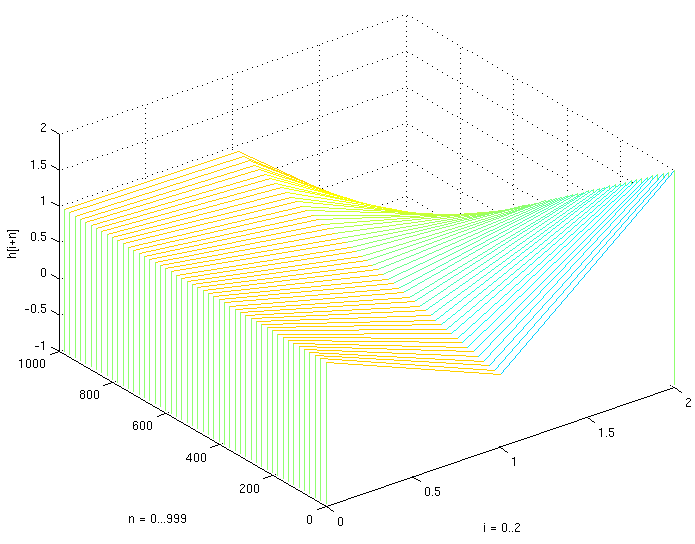
\includegraphics[width=16cm]{./plots/waterfall.png}
 % waterfall.png: 1400x920 pixel, 90dpi, 39.51x25.97 cm, bb=0 0 1120 736
 \caption{Wasserfall Darstellung der Impulsantwort}
 \label{fig:waterfall}
\end{figure}

\subsection{(c) Adaptiver Filter ohne Rauschen}

In der Abbildung \ref{fig:c_20} bzw. \ref{fig:c_50} wurden die Koeffizienten
des ``unbekannten'' Systems mit den Koeffizienten des Adaptiven Systems verglichen.

Dabei kann man erkennen, dass bei einem gr��erem M das unbekannte System besser angen�hert werden kann.
Die Koeffizienten haben wie in den Abbildungen ersichtlich eine kleinere Varianz. Das ganze ist nat�rlich
logisch, da l�ngere Bl�cke verarbeitet werden.

Nachteil eines gr��eren M ist ein etwas gr��erer Berechnungsaufwand.
Ein weiterer Nachteil welcher zwar hier nicht ersichtlich ist, dass die Filterkoeffizienten
bei schnelleren �nderungen von $\textbf{h}[n]$ nicht mitkommen.

\subsection{(d) Adaptiver Filter mit Wei�em Rauschen}
In den Abbildungen \ref{fig:d_20} bzw. \ref{fig:d_50} ist zu erkennen, dass das Hinzuf�gen von
Wei�em Rauschen keinen wesentlichen Unterschied bringt. Die Abweichung von den idealen
Koeffizienten ist nat�rlich etwas gr��er.

\subsection{(e) Adaptiver Filter mit vom Eingang abh�ngigem $\nu[n]$}
In den Abbildungen \ref{fig:e_20} bzw. \ref{fig:e_50} ist zu erkennen,
dass die durch das Adaptive Filter angen�herten Koeffizienten einen Offset zu den idealen Koeffizienten haben.
Dies liegt daran, dass $\nu[n]$ abh�ngig vom Eingang $x[n]$ ist.

Betrachtet man die Gleichung:
\begin{equation}
 \nu[n] = 1/2 \cdot (x[n] + x[n-1])
\end{equation}

so f�llt auf, dass $\nu[n]$ aus einem Filter mit den Koeffizienten $[0.5;0.5;0]$ aus $x[n]$ erzeugt werden kann.
Dies spiegelt sich auch in den Koeffizienten des Adpativen Filters wieder. Somit l�sst sich der
``Offset'' der Koeffizienten in den Abbildungen \ref{fig:e_20} bzw. \ref{fig:e_50} erkl�ren.







\newpage

\begin{figure}[ht!]
 \centering
 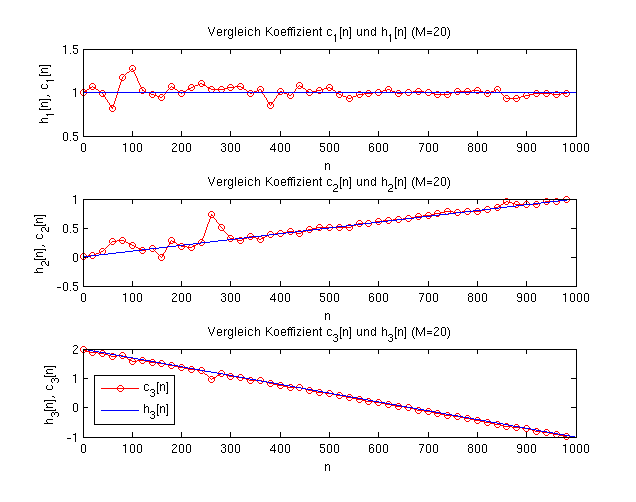
\includegraphics[width=13.5cm]{./plots/c_coefficients_M20.png}
 % waterfall.png: 1400x920 pixel, 90dpi, 39.51x25.97 cm, bb=0 0 1120 736
 \caption{Koeffizienten des Filters mit M=20, $v[n] = 0$}
 \label{fig:c_20}
\end{figure}

\begin{figure}[ht!]
 \centering
 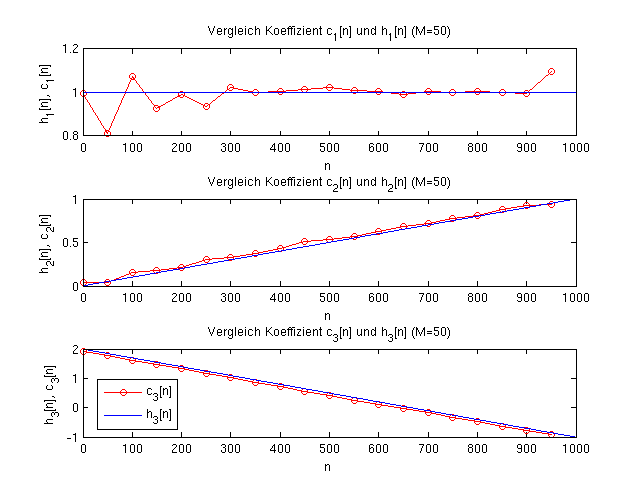
\includegraphics[width=13.5cm]{./plots/c_coefficients_M50.png}
 % waterfall.png: 1400x920 pixel, 90dpi, 39.51x25.97 cm, bb=0 0 1120 736
 \caption{Koeffizienten des Filters mit M=50, $v[n] = 0$}
 \label{fig:c_50}
\end{figure}


\begin{figure}[ht!]
 \centering
 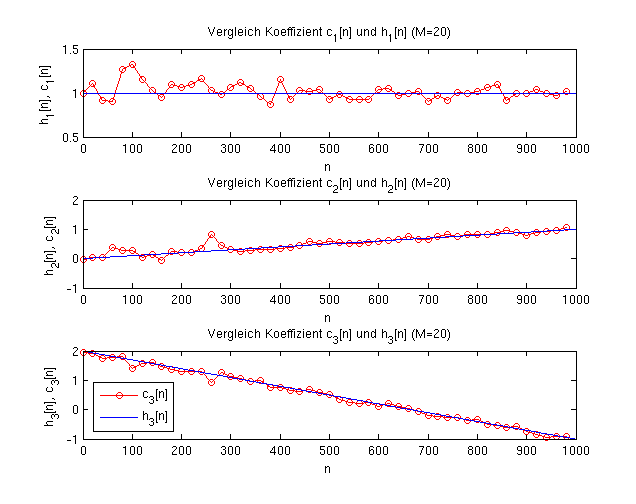
\includegraphics[width=13.5cm]{./plots/d_coefficients_M20.png}
 % waterfall.png: 1400x920 pixel, 90dpi, 39.51x25.97 cm, bb=0 0 1120 736
 \caption{Koeffizienten des Filters mit M=20, $v[n] = $ zero mean white noise with Variance = 0.5}
 \label{fig:d_20}
\end{figure}

\begin{figure}[ht!]
 \centering
 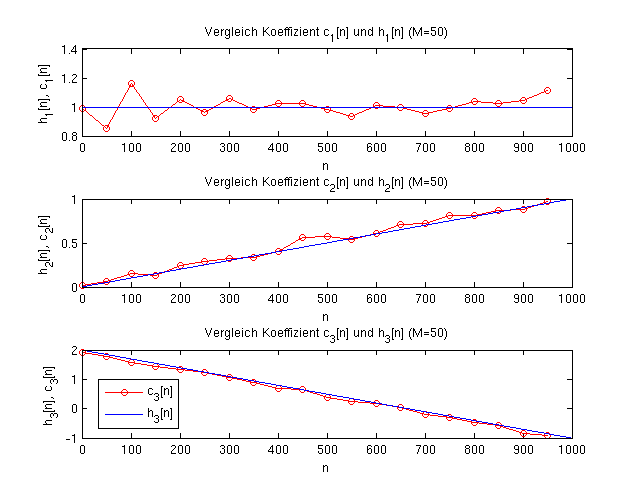
\includegraphics[width=13.5cm]{./plots/d_coefficients_M50.png}
 % waterfall.png: 1400x920 pixel, 90dpi, 39.51x25.97 cm, bb=0 0 1120 736
 \caption{Koeffizienten des Filters mit M=50, $v[n] = $ zero mean white noise with Variance = 0.5}
 \label{fig:d_50}
\end{figure}

\begin{figure}[ht!]
 \centering
 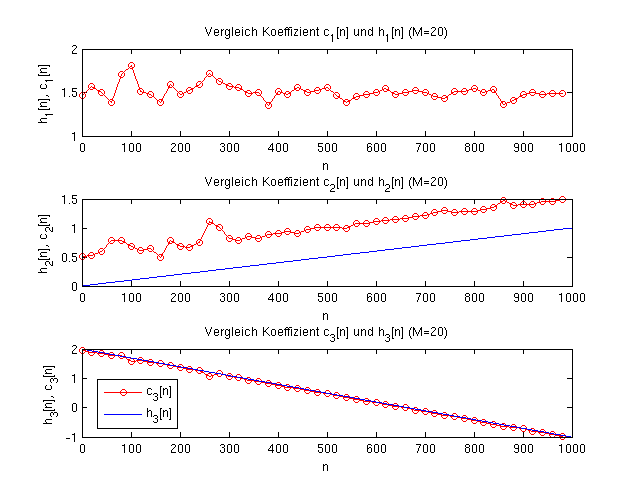
\includegraphics[width=13.5cm]{./plots/e_coefficients_M20.png}
 % waterfall.png: 1400x920 pixel, 90dpi, 39.51x25.97 cm, bb=0 0 1120 736
 \caption{Koeffizienten des Filters mit M=20, $v[n] = 0.5\cdot (x[n] + x[n-1]$}
 \label{fig:e_20}
\end{figure}

\begin{figure}[ht!]
 \centering
 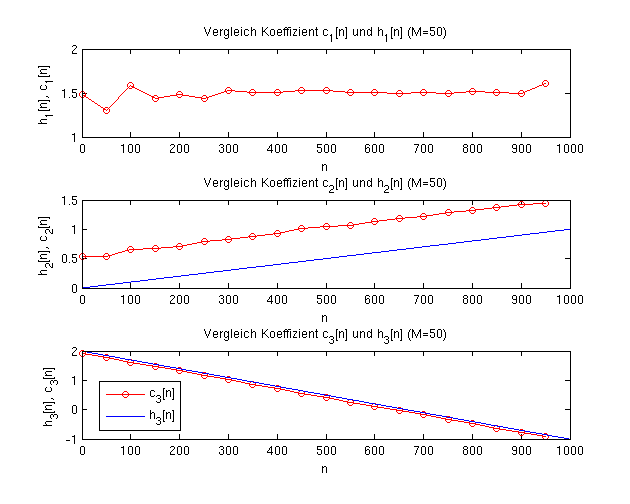
\includegraphics[width=13.5cm]{./plots/e_coefficients_M50.png}
 % waterfall.png: 1400x920 pixel, 90dpi, 39.51x25.97 cm, bb=0 0 1120 736
 \caption{Koeffizienten des Filters mit M=50, $v[n] = 0.5\cdot (x[n] + x[n-1]$}
 \label{fig:e_50}
\end{figure}